\section{Related Work}
Massive model rendering is a well studied problem in computer graphics. Most of
the early works focused on increasing the rendering efficiency. At that time
the fundamental problem was not fitting the model into main memory, but
fully utilizing the speed of the graphics cards. Hence these works provided
solutions to reduce the number of primitives to be rendered while maintaining
the visual fidelity. These solutions included level-of-detail for geometric
models \cite{Luebke02}, progressive level of detail
\cite{Hoppe:98b,Hoppe:97,Hoppe:96,SG:01}, and image based simplification
\cite{ACWBZEHHSBWBM:99}. Soon thereafter the size of main memory became the
bottleneck in handling ever increasing sizes of the model. Hence memory-less
simplification techniques \cite{LT:99}  and other out-of-core rendering systems
\cite{Silva02,VM:02} emerged in which just the limited amount of required data
that needs to be processed and rendered was brought from the secondary storage
to main memory. \\
\\
The speed at which this data
could be brought from the secondary to main memory in these out-of-core
algorithms is limited by the data bus speed, disk seek time, and data transfer
time. These limitations could be ameliorated to some extent by
better cache utilization that would increase the utilization of data that is
brought to main memory and thus reduce the number of times the disk read is
initiated. This meant that subsequent works focused on cache aware
\cite{ssdpaper} and cache oblivious data layouts
\cite{cacheobliviouslayout,YOON:2006:MeshLayout} on the disk to reduce the
data fetch bottleneck. Our work falls under this class of algorithms that
reduces the data fetch time. \\
\\
Redundancy based data layouts were mentioned in
\cite{Patterson88,singleseeklayout,optimizingredundancy} as potential solutions
to the problem of reducing seek time. In particular
\cite{optimizingredundancy} presented a data layout algorithm based on integer programming specifically useful in walkthrough applications that models the seek time as the number of seeks to the beginning of different data groups. These data groups are the ones to be fetched to render one frame. However, there were major drawbacks. First, although it provides the data units to be grouped and considered as one seek, for each seek it does not provide a data layout.
This is because it does not relate one data group with another.
Such an approach could easily result in unnecessary data
block duplications since groups of data units can overlap with each other and only one copy of the common data unit may be required. There is no mechanism in the integer programming solver to detect whether this redundancy is necessary because of some scene context or simply created blindly due to local optimization. The redundancy minimization is thus not modeled after
physical representation of the data layout on the disk. The second major
drawback is that the model for seek time is also not based on physical reality.
Typically, seek time depends on the relative distance on the disk between the
last data unit accessed and the data unit currently being requested. However,
in \cite{optimizingredundancy}, seek time is simplistically modeled,
 as number of data groups accessed for each fetch
independent of the number of data units between these data groups. Irrespective of whether the requested data blocks are adjacent to
each other or far apart, this model would assign the same cost for both
layouts. Our approach
aims to address these issues. 


\begin{figure}[t]
  \centering
  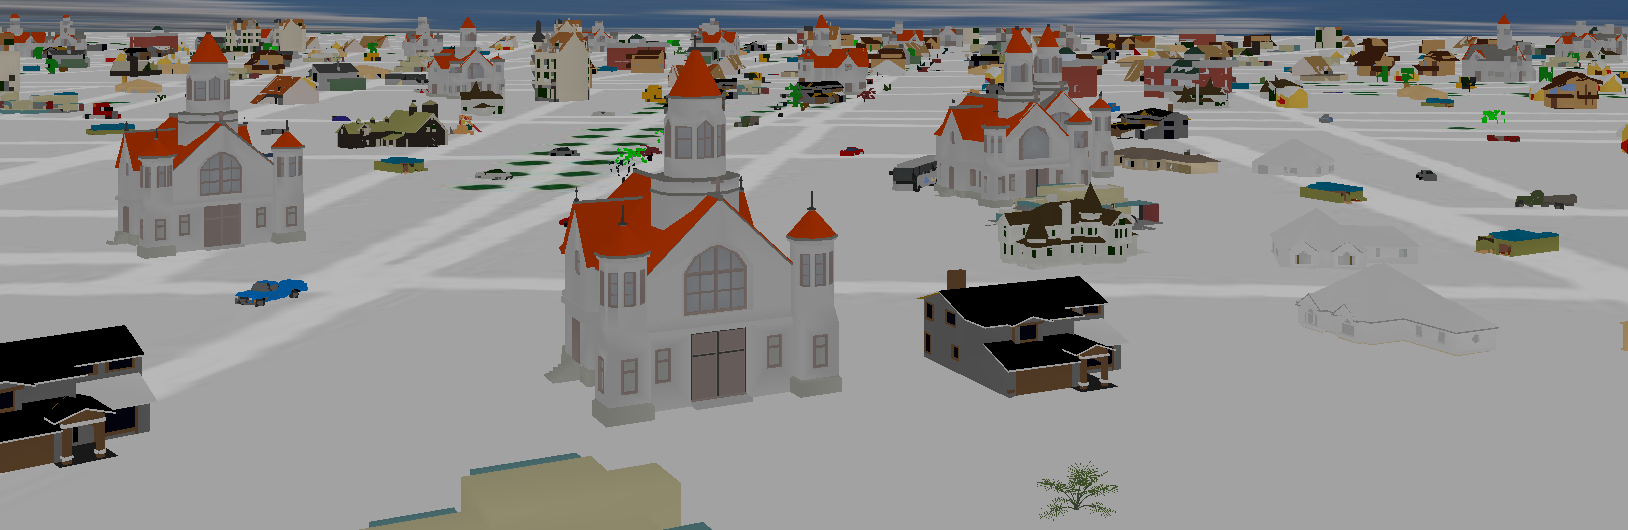
\includegraphics[width=\columnwidth]{city.png}
  \caption{City model: 110 million triangles, 6 GB }
  \label{fig:model1}
\end{figure}


